\documentclass[../main/main.tex]{subfiles}
\begin{document}
\chapter[Multi-dimensional integration in HEP]{Multi-dimensional integration in HEP}
In this chapter we focus at first on Monte Carlo techniques applied to the problem of multi-dimensional numerical integration.
We discuss the two main methods which involve importance sampling and stratified sampling.
Secondly, we give a brief overview on High Energy Physics (HEP) arguments, such as the the $S$-matrix formalism, Feynman diagrams and Quantum Chromodynamics, with particular attention 
on the computation of physical observables as a series of perturbative terms which involve high-dimensional integrals.
Finally, we present the state-of-the-art of  MC integration applied to HEP and discuss the current problems and limitations which
is facing the High-Luminosity LHC programme at CERN.

\section[MC methos for multi-dimensional integration]{Monte Carlo methods for multi-dimensional integration}
Monte Carlo (MC) integration methods are powerful tools which can provide the answer to a 
problem by simply running a simulation of the system under study.
In the field of multi-dimensional integration techniques, MC methods are the solution of choice, since contrary 
to the standard numerical integration formulas  the error on the integral does not scale with the dimension \cite{Press:1992zz}. 


\subsection{A first example of Monte Carlo integration}
In the case of multi-dimensional integration we are interested in performing the
integral:
\begin{equation}
	I = \int_{V}   f(\textbf{x}) d \textbf{x} \ , 
\end{equation}
where $V$ is the domain of the integration and $f$ is a function of $n$ variables 
$\textbf{x} = (x_1,x_2, ..., x_n)$.

When performing the integral $I$ the simulation comes down to a sampling of the integrand function.
First we need to generate a set of random points $\textbf{x}_i$ which belong to the integration domain $V$.
The simplest way to perform the sampling is to pick random points uniformly distributed 
in the volume $V$.

An estimate of the integral using $N$ random points can be given as
\begin{equation}
	I \approx I_{\text{MC}} = V \frac{1}{N} \sum_{\textbf{x}_i \in V} f(\textbf{x}_i) = V \langle f \rangle \ ,
\end{equation}
where $\langle f \rangle$ denotes the arithmetic average of the function $f$.

$I_{\text{MC}}$ is a random number, whose value depends on the sampled points, whose mean 
is given by the exact value of the integral $I$ and the variance is given by
\begin{equation}
	\label{variance}
	\sigma^2_I = \frac{1}{N} \big[ V \int_{V}   f^2(\textbf{x}) d \textbf{x}  - I^2 \big] \ .
\end{equation}

This variance is asymptotically related to the variance of the random value $I_{\text{MC}}$, therefore
we can estimate the value of $\sigma^2_I$ in the limit of large $N$ as
\begin{equation}
	\label{sigma_MC}
	\sigma^2_I \approx \sigma^2_\text{MC}  = \frac{1}{N-1} \Big[ 
	V^2 \langle  f^2 \rangle 
	- I^2_{\text{MC}}\Big] \ .
\end{equation}

In both cases we observe that the standard deviation decreases as the sample increases 
as $N^{-\frac{1}{2}}$ regardless of the dimension of the volume $V$. This is a remarkable feature of MC integration which differs from the standard quadrature techniques where the error 
increases with the dimension.

MC integration can also deal with the complicated boundaries problem of quadrature integration.
Suppose that we need to integrate a function $h$ over some complicated region $H$, for which the 
random sampling becomes challenging. 
In this particular case we can easily overcome such problem by replacing the region $H$ with a new volume 
$G$ that includes $H$ and it is more suitable for the process of sampling. After that all we need to do is to replace also 
the function $h$ with a new function $g$ defined as:
\begin{equation}
	g(\textbf{x}) = \begin{cases}
		h(\textbf{x}) &\text{ if $\textbf{x} \in H$} \\
		0 &\text{ if $\textbf{x} \in G - H$} \ .
	\end{cases}
\end{equation}

Obviously one should try to make the new region $G$ not too oversized with respect to $H$, because every 
point $\textbf{x} \in G - H$ will contain no information about the integrand. Therefore the number of 
effective points used during the sampling $N$ will reduce by raising the error in Eq.~\eqref{sigma_MC}.

This first MC integrator has a few disadvantages:
\begin{enumerate}
\item We have already observed that the error decreases as the square root of the number of sampled points, 
	this implies that if the accuracy requirements are high we will need to increase the size of the sampling. 
	Dealing with huge sizes of sampled points could be, even for a computer with large memory and a fast processor, 
	challenging and we expect that the process of sampling could take a significant amount of time.
	\item One will probably have to work with large samples, even if the accuracy requirements are modest, when
	the dimensionality of the integration domain is high. The reason being that if the integrand function is peaked in a small
	region compared to the volume $V$, we will need to generate more random points to make sure that the peak is correctly 
	identified; such process of finding the peaks becomes more challenging in large number of dimensions.
	This can be seen for example by considering the ratio of the volume of a $D$ dimensional hypersphere with unity radius to the $D$ dimensional hypercube with a side of twice the unity radius , which vanishes as the $D$ goes to infinity as:
	
	\begin{equation}
		\frac{V_{\text{hypersphere}}}{V_{\text{hypercube} }} = \frac{1}{2^D} \frac{\pi^{\frac{D}{2}}}{\Gamma\big(\frac{D}{2} + 1\big)} \approx  \bigg( \frac{\sqrt{\pi}}{2} \bigg)^D \xrightarrow{D \rightarrow  \infty} 0 \ ,
	\end{equation}
	where $\Gamma(x)$ denotes the famous Gamma function.
	
	In literature this phenomenon is known as the \emph{curse of dimensionality}.
\end{enumerate}




\subsection{Reducing the variance}
\label{redu_var}
In the field of MC integrators the main focus is to improve the error estimate in order to achieve more precise results using less events. Over the years and also lately with the advent of Machine Learning, several techniques have been proposed, implemented and applied to solve complex multi-dimensional integrals \cite{Lepage:2020tgj, Carrazza:2020rdn, unknown}.

In literature there are two main ways of reducing the variance: importance sampling and stratified sampling.

\subsubsection{Importance Sampling}
In the naive MC integrator the sampling was performed by picking random points uniformly distributed in the integration volume. 
We have already discussed that if the integrand has a peak in a small region it will be challenging to find it especially because we are selecting points from a uniform distribution. 

Suppose that the points $\textbf{x}_i$ are chosen within the integration volume $V$ with a probability density $p$ correctly normalized:
\begin{equation}
	\label{normalization}
	\int_{V} \;  p(\textbf{x})  d \textbf{x}  = 1 \ .
\end{equation}
We can calculate the integral $I$ as:
\begin{equation}
	\label{samplig2}
	I = \int_{V}   f(\textbf{x})  d \textbf{x}  =\int_{V}   \frac{f(\textbf{x})}{ p(\textbf{x})} p(\textbf{x})  d\textbf{x}
	= \int_{V}  \frac{f(\textbf{x})}{ p(\textbf{x})} dP(\textbf{x}) \ ,
\end{equation}
where in the last step we used the transformation $d\textbf{x} = dP(\textbf{x})/p(\textbf{x}) $, with $P(\textbf{x})$ the 
cumulative distribution of  $p(\textbf{x}) $.
\newline
From Eq.~\ref{samplig2} we can deduce that in order to compute the integral $I$, instead of using a uniform sampling of the function $f$,
we can also perform a non-uniform sampling of the function $f/p$ in the same integration volume $V$.
\newline
The integral and the relative error will be given by \cite{unknown}:
\begin{equation}
	I \approx I_{\text{MC}}  = V \langle f/p \rangle_P \ ,
\end{equation}
\begin{equation}
	\label{sigma_IP}
	\sigma^2_I \approx \sigma^2_\text{MC} = \frac{V^2}{N-1} \bigg[\langle (f/p)^2 \rangle_P - \langle f/p \rangle^2_P \bigg] \ ,
\end{equation}
where $\langle \rangle_P$ denotes the average taken with respect to the non-uniform distribution $p(\textbf{x})$.

This is the concept of \emph{importance sampling}: by changing the distribution of the sampling we can reduce the variance by choosing
a suitable $p(\textbf{x})$ \cite{Lepage:1977sw, Lepage:2020tgj, unknown}.

What is the best choice for the sampling density $p$?
It can be shown that by minimizing the variance, as a functional of sampling density $p$, the optimal choice for $p$ is to be proportional 
to $|f|$. This choice is not surprising, in fact by replacing $p$ with $|f|$ in Eq.~\ref{sigma_IP} we get a vanishing variance.
Moreover, in order to satisfy the normalization requirement in Eq.~\ref{normalization} the exact solution for $p$ is:
\begin{equation}
	p = \frac{|f|}{\int_V |f| d\textbf{x}} \ .
\end{equation}
\newline
As we can see we arrive at a paradox since the optimal sampling density requires the knowledge of $\int_V |f(\textbf{x})| d\textbf{x}$ which is the integral that we are trying to compute!
\newline
Therefore to minimize the variance the aim is to find a function $p$ that resemble the shape of the integrand function $f$, this is usually done 
using adaptive recursive strategies which can provide a better sampling distribution using the previously sampled points.
\subsubsection{Stratified Sampling}
Another technique which is a standard one in literature is based on the idea of  "stratified sampling" \cite{Press:1989vk, Press:1992zz}.
We have already observed that we can estimate the variance of our integral by computing the variance of the random variable $I_{\text{MC}}$; we can exploit this relation by focusing on the average value of the function $f$ over the domain $V$, denoted by $\llangle  f \rrangle $, and the corresponding MC estimate using an uniform sampling $ \langle f \rangle$:
\begin{equation}
	\llangle  f \rrangle = \frac{1}{V} \int_V f(\textbf{x}) d\textbf{x} \quad ,  \quad 
	\langle f \rangle = \frac{1}{N} \sum_{\textbf{x}_i} f(\textbf{x}_i) \ .
\end{equation}
We can now rewrite Eq.(\ref{sigma_MC}) as  
\begin{equation}
	\text{Var}( f ) \equiv \llangle f^2 \rrangle - \llangle f \rrangle ^2 = \frac{\langle f^2 \rangle - \langle f \rangle^2}{N} \equiv \frac{\text{Var}(\langle f \rangle )}{N} \ .
\end{equation}

Suppose we divide the volume $V$ into two subvolumes $V_a$  and $V_b$, chosen equal and disjoint, and we sample exactly $N/2$ points in each subvolume. We can formulate another estimator for the mean value of the function, $\llangle f \rrangle $ as the arithmetic mean between the sample average
in the two half-regions:
\begin{equation}
	\label {SS f}
	\langle f  \rangle ' \equiv \frac{1}{2} (  \langle f \rangle_a + \langle f \rangle_b ) \ ,
\end{equation}
where $\langle \rangle_a$ denotes the MC estimate of the function for the $N/2$ points belonging to the subvolume $V_a$ and similarly for $\langle \rangle_b$.
The variance of the estimator in Eq.(\ref{SS f}) can be easily computed as:
\begin{eqnarray}
	\text{Var}(\langle f \rangle ') &= \dfrac{1}{4}  \big[  \text{Var}(\langle f \rangle_a) +\text{Var}(\langle f \rangle_b)  \big]  \\
	&= \dfrac{1}{4} \bigg(  \dfrac{\text{Var}_a(f)}{N/2} +\dfrac{\text{Var}_b(f)}{N/2} \bigg) \\
	&= \dfrac{1}{2N} \big[ \text{Var}_a(f) + \text{Var}_b(f)\big] \label{var_stratified} \ ,
	\label{ SS var}
\end{eqnarray}
where $\text{Var}(\langle f \rangle)_{i} = \llangle f^2 \rrangle_i - \llangle f \rrangle^2_i$ denotes the variance of $f$ limited to the subvolume $V_i$.

One could ask how the variance in subvolumes $V_i$ is related to the variance of $f$ in the whole integration domain $V$. This can be easily done using the additivity of the integral, the result is known in literature as the parallel axis theorem:
\begin{equation}
	\text{Var}(f) = \frac{1}{2} [ \text{Var}_a(f) + \text{Var}_b(f)] + \frac{1}{4} ( 
	\llangle f \rrangle_a - \llangle f \rrangle_b)^2 \ .
\end{equation}

As we can see, the stratified sampling gives a variance which is always equal or smaller than the variance of the naive MC integrator. In particular whenever the function $f$ behaves differently in 
the two regions $V_a$ and $V_b$, the variance of $f$ increases as $ ( 
\llangle f \rrangle_a - \llangle f \rrangle_b)^2$ and such difference does not affect the $\text{Var}(\langle f \rangle')$ given by Eq.~\ref{ SS var}.
\newline
We can generalize the previous formulas by adding the possibility to sample a specific number of 
points from each subvolume. Considering again the subvolumes $V_a$ and $V_b$ we can suppose 
to sample the first one with $N_a$ points and the second one with $N_b$ with the constraint that $N = N_a + N_b$. 
\newline
It can be shown that in this case the variance is minimized when \cite{Press:1989vk}:
\begin{equation}
	\frac{N_a}{N} = \frac{\sqrt{\text{Var}_a(f)}}{\sqrt{\text{Var}_a(f)}+
		\sqrt{\text{Var}_b(f)}} \ .
\end{equation}

Consequently, we observe that the number of sample in a particular subvolume is proportional to the standard deviation of the samples in that subregion, which is quite expected. If there is a region with high variance we will need more points in order to have a better knowledge of the behaviour of the 
integrand function.
\newline
With the aim of taking full advantage from stratified sampling, the standard procedure is to divide
the integration domain in several subvolumes each one with a different number of samples. Again by minimizing the variance we find that the number of samples in each subregion must be proportional
to the standard deviation in that particular subregion.
\newline
Stratified sampling can struggle in higher dimensions due to the large number of subregions.
In fact if we divide the integration volume in $M$ subvolumes for each dimension we will end up with a total of $M^d$  total subregions. Considering that in order to compute the variance in each region we need at least two points, we will need a total of $2 M^d$ sampled points, which can become challenging.



\section{HEP and multi-dimensional integration}
One of the main fields of physics which requires computing multi-dimensional integrals is High Energy Physics (HEP).
In this section we give a brief overview on some aspects of quantum field theory \cite{Peskin:1995ev, Schwartz:2017hep}, in particular we show that a prediction for a physical
observable can be made as a series of perturbative terms which involve the evaluation of high dimensional integrals.

Finally, we present shortly the quantum theory of strong interactions known as Quantum Chromodynamics (QCD) \cite{Collins:2011zzd, Muta:2010xua, Ellis:1991qj, Skands:2012ts}.


\subsection{Cross Section and Decay Rates}
The experiments performed at the Large hadron Collider (LHC) \cite{Aad:2008zzm, Chatrchyan:2008aa} are aimed at probing the behaviour of elementary particles, which can be considered in a 
relativistic regime due to the high energies required. These are usually scattering experiments in which two beam of particles with well defined momenta collide creating new particles which are detected and measured.

The probability of finding a particular final state can be expressed in terms of a physical observable, the cross section.
Suppose that we have two species of particle, $\mathcal{A}$, at rest with density $\rho_\mathcal{A}$ , and $\mathcal{B}$ moving at velocity $v$ towards $\mathcal{A}$ with density $\rho_\mathcal{B}$. Imagine also that we can measure the length of the two beam of particles $l_\mathcal{A}$ and $l_\mathcal{B}$. 

\begin{figure}[h]
	\centering
	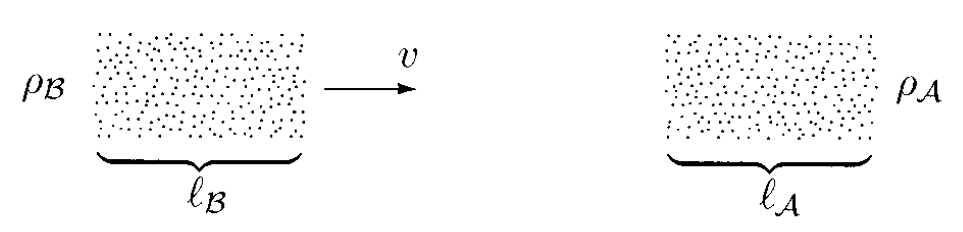
\includegraphics[width=12cm]{../images/peskin.png}
	\caption{Symbolic representation of a scattering process. Image from Ref.~\cite{Peskin:1995ev}.}
	\label{Potential}
\end{figure}

We expect that the total number of scattering events must be proportional to the cross-sectional area $A$ common to the two beams and all the previous quantities; the cross section, $\sigma$, is defined indeed as:
\begin{equation}
	\sigma \equiv \frac{\text{ Number of scattering events}}{A \rho_\alpha \rho_\beta  l_\alpha l_\beta} \ .
\end{equation}
We also wish to measure the momenta of the outgoing particles, which are expected to be infinitesimal. In order to do so we can define a differential cross section $ d \sigma/(d^3p_1...d^3p_n)$ such that:
\begin{equation}
	\int_\Omega \frac{ d \sigma}{d^3p_1...d^3p_n}d^3p_1...d^3p_n = \sigma|_\Omega \ ,
\end{equation}
where $\sigma|_\Omega$ gives the cross section for scattering in the region of final-state momentum space $\Omega$. Obviously the final state momenta are not all independent.

Firstly, the total four-momentum of the incoming particles must be equal to the total momentum of the outgoing particles by four-momentum conservation. Secondly, each particle detected will have a given mass (or zero for massless ones) which fixes the four momentum components, $p_i^2 = m_i^2$.

The majority of the particles produced during the collision are unstable, that is, the lifetime $\tau$ of 
such particles is so short that they cannot be detected by the experimental apparatus.
Nevertheless we know that an unstable particle decays in other particle species some of which can be detected. 
For an unstable particle $\delta$  we can define a new observable, the decay rate $\Gamma$ defined as 
\begin{equation}
	\Gamma = \frac{\text{Number of decays per unit time}}{\text{Number of  $\delta$  particles present }} \ .
\end{equation}
The lifetime can be computed as the reciprocal of the sum of its decay rates into all possible final states.

This two physical observables can be computed theoretically by using the scattering matrix $S$ firstly introduced by Heisenberg.
\subsection{The $S$-matrix formalism}
When particles collides during a scattering experiments they interact according to the fundamental
interactions describes by the Standard Model (SM).
In particular the SM is a quantum field theory that explains how three of the four fundamental forces (strong, weak and electromagnetic) can be described through the exchange of particles called bosons.
\newline
The beams of incident particles in a quantum field theory is treated as a quantum state $\ket{\phi_A\phi_B}_{\text{in}}$, in the same way the final state detected will be denoted by $\ket{\phi_1 \phi_2 \dots \phi_n}_{\text{out}}$. 
Both, the initial and final states, can be expressed as linear superpositions of eigenstates of the free theory, i.e.with definite momenta, constructed in the far past and in the far future respectively.
For example for the final state we can write:
\begin{equation}
	\ket{\phi_1 \phi_2 ...\phi_n}_\text{out} =\bigg( \prod_{i=1}^{n}\int
	 \frac{d^3 p_i}{(2 \pi)^3}
	\frac{\phi_i(\textbf{p}_i)}{\sqrt{2 E_i}} \bigg) \ket{\textbf{p}_1\textbf{p}_2...\textbf{p}_n}_\text{out} \ .
\end{equation}
The probability  of scattering, which is connected to the overlap between the initial and final states, can be related to the transition amplitudes between the eigenstates of momenta created in the far past \emph{in} and in the far future \emph{out}
\begin{equation}
	{}_\text{out}\braket{\textbf{p}_1\textbf{p}_2 ... \textbf{p}_n | \textbf{k}_1 \textbf{k}_2 }_\text{in} = \lim_{T \to \infty} \braket{\textbf{p}_1\textbf{p}_2 ... \textbf{p}_n |e^{- i H T} |\textbf{k}_1 \textbf{k}_2 } \equiv \braket{\textbf{p}_1\textbf{p}_2 ... \textbf{p}_n |S |\textbf{k}_1 \textbf{k}_2 } \ ,
\end{equation} 
where we have written explicitly the time evolution. As we can see the braket between the two asymptotic states can be rewritten as the braket between two momenta eigenstates by the limit of a sequence of unitary operators that is called \emph{S-matrix}:
\begin{equation}
	{}_\text{out}\braket{\textbf{p}_1\textbf{p}_2 ... \textbf{p}_n | \textbf{k}_1 \textbf{k}_2 }_\text{in} =  \braket{\textbf{p}_1\textbf{p}_2 ... \textbf{p}_n |S |\textbf{k}_1 \textbf{k}_2 } \ .
\end{equation} 
If we are studying a non-interacting theory the $S$ matrix is simply the identity matrix, since state of
definite momentum are eigenstate of the free-field Hamiltonian, which are orthogonal. If we consider an interacting theory we can rewrite $S$ as the identity matrix plus a non-trivial matrix $T$: $S = \textbf{1}+ i T$.
\newline
In literature the matrix element of the $T$ matrix is written as:
\begin{equation}
	\label{first matrix element}
	\braket{\textbf{p}_1\textbf{p}_2 ... \textbf{p}_n |i T | \textbf{k}_1 \textbf{k}_2 } \equiv 
	(2 \pi)^4 \delta^{(4)}\big(k_1+k_2- \sum_{i=1}^n p_i\big) \cdot i \mathcal{M} \ ,
\end{equation}
where we introduced the invariant matrix element $\mathcal{M}$ by removing a factor that reflects the four-momentum conservation.
The previous separation is useful since $\mathcal{M}$ contains all the information regarding the interaction, while all the other factors depends merely on the kinematics of the process.

In particular, it can be shown that the differential cross section $d\sigma$ can be computed using the square modulus of the invariant 
matrix element and the kinematic quantities of the particles involved in the collision:
\begin{equation}
	\label{sigma}
	d \sigma = \frac{1}{4 E_A E_B |v_A - v_B|} \  d\Pi_n \times |\mathcal{M}(k_A, k_B \to p_1, ..., p_n)|^2  \ ,
\end{equation}
where $ |v_A - v_B|$ is the relative velocity between the two beams.  To compute the cross section $\sigma$ we need to perform the integral over the final momenta, which is of the form
\begin{equation}
	\int d\Pi_n  = \bigg( \prod_{i=1}^{n}\int
	\frac{d^3 p_i}{(2 \pi)^3}
	\frac{1}{2 E_i} \bigg) (2\pi)^4 \delta^{(4)}\big(k_A+ k_B- \sum_{i=1}^n p_i\big) \ ,
\end{equation} 
which corresponds to an integral involving $3n$ variables where $n$ is the number of particles in the final state.

There is also a formula to compute the differential decay rate $d\Gamma$; it can be obtained considering an initial state with a single
unstable particle in his rest frame that decays in $n$ outgoing particles.
\begin{equation}
	d\Gamma = \frac{1}{2 m_A} \bigg( \prod_{i=1}^{n}
	\frac{d^3 p_i}{(2 \pi)^3}
	\frac{1}{2 E_i} \bigg) (2\pi)^4 \delta^{(4)}\big(k_A- \sum_{i=1}^n p_i\big) \times |\mathcal{M}(k_A \to p_1, ..., p_n)|^2 \ .
\end{equation}
We have two equations to compute the differential cross section and the differential decay rate which involve the square modulus of 
the invariant matrix element $\mathcal{M}$. In the next subsection we show how $\mathcal{M}$ can be calculated pertubatively using Feynman diagrams.

\subsection{Feynman diagrams}
The invariant matrix element $\mathcal{M}$ was firstly introduced in Eq.~\ref{first matrix element} in the overlap between two momenta
eigenstates with the $S$ matrix.
Such matrix has an exact solution which is expressed as a series of terms, known as Dyson expansion:
\begin{equation}
	\label{S}
	S = \sum_{n = 0}^{\infty} S^{(n)} = \sum_{n = 0}^{\infty} =  \frac{(-i)^n}{n!}\idotsint d^4 x_1 ... d^4 x_n \mathcal{T}\{ \mathcal{H}_I(x_1) \dots \mathcal{H}_I(x_n) \} \ ,
\end{equation}
where $\mathcal{T}\{ \mathcal{H}_I(x_1) \dots \mathcal{H}_I(x_n) \}$ denotes the normal ordered product of the interacting 
Hamiltonian densities $ \mathcal{H}_I(x_1) \dots \mathcal{H}_I(x_n)$ and the integral is over all space-time.

The expansion is reliable only if we can treat the interacting hamiltonian density, $\mathcal{H}_I$, as a perturbation which is the case for 
the majority of the theories studied. For example, in QED the interaction is proportional to the fine structure constant $\alpha \approx 1/137$, thus the perturbative expansion makes sense.

Thanks to Wick's theorem it is possible to rewrite the time-ordered product in a different way which can be represented graphically using Feynman diagrams. 
To be more specific Feynman diagrams are graphs in which each part from the lines to the vertices is linked to a mathematical expression.
The set of rules that allows us to pass from the pictorial representation to the correct mathematical formula are called Feynman rules, and
are easily obtainable from the Lagrangian of the theory.

As for the matrix $S$, also the matrix element $\mathcal{M}$ can be written as a perturbative expansion:
\begin{equation}
	\label{exp M}
	\mathcal{M}= \sum_{n = 1}^{\infty} \mathcal{M}^{(n)} \ ,
\end{equation} 
where the contribution $\mathcal{M}^{(n)} $ comes from the $n$th order perturbation term $S^{(n)}$ and can be obtained by drawing 
all topologically different, connected Feynman diagrams which contain $n$ vertices and the correct number of external lines.

Among the different diagrams there are some which may contain loop lines, which correspond to quantum corrections.
 The Feynman rules tell us that for each loop line we must add an integration over the momentum $k$ of that line, since such momentum is not fixed by the process.

The perturbative expansion of $\mathcal{M}$ can be seen as a sum of integrals with increasing dimension. The first contribution comes 
from the diagrams that contain no loops, which is referred as \emph{tree-level} since such diagrams obey the definition of a tree in graph
theory. The second contribution will come from the one-loop diagrams in which the dimension of the integral increases 
since we are also integrating over the loop momentum. By repeating this process we can express $\mathcal{M}$ as:
\begin{equation}
	\mathcal{M}=\mathcal{M}^{\text{tree}} + \mathcal{M}^{\text{1-loop}} + \mathcal{M}^{\text{2-loop}} + \dots \ .
\end{equation}

It is well known in the field of quantum field theories that the diagrams which involves loop corrections can lead to divergent contributions, in the limit where the momenta of the loop particles become large. These divergences are known as ultra-violet (UV) divergences and in renormalizable theories, like QCD, they can be removed by a modification of the continuum limit, at least in perturbation theory.
If the considered theory is \emph{renormalizable} there are specific techniques to handle this type of divergences which belong to the 
field of \emph{renormalization}.

Infra-red IR divergences also appear in perturbation theory for the $S$-matrix of theories such as QCD and QED that have massless fields.
This type of infinities arise when we consider radiative corrections to the tree-level diagram, i.e.\ when extra particles with vanishing energy are emitted.

For example in QED we can start from the process $e^- e^+ \to \mu^+ \mu^-$ at tree-level and then consider a radiative correction which 
involves the emission of a photon from one of the two final-state quarks. The second order radiative correction will involve the emission of 
two photons and so on. Finally we can arrive at an expression to include all this radiative corrections of the form:
\begin{equation}
	\mathcal{M}^{\text{inclusive}} = \mathcal{M}^{\text{tree}} + \mathcal{M}^{\text{1-leg}} + \mathcal{M}^{\text{2-leg}} + \dots \ ,
\end{equation}
where $\mathcal{M}^{\text{1-leg}}$ corresponds to the emission of a single particle,  $\mathcal{M}^{\text{2-legs}}$ emission of two
particles and so on.
We can observe that also these sequences involves integral of increasing dimensions since by adding one extra particle to the final states 
we go from an $3n$ dimensional space to a $3n + 3$ space, always considering a final state of $n$ particles.

IR singularities also appear in loop diagrams and thanks to the Kinoshita-Lee-Nauenberg (KLN) theorem it is possible to prove that the singularities of the real emissions and those one of the loop diagrams cancel each other out  order by order in perturbation theory.

We have therefore shown that when computing a physical observable in quantum field theory we obtain a perturbative expansion which 
involves both loop diagrams and radiative correction which is finite. We can denote the first non vanishing term in this series as the 
\emph{leading order} (LO) term, the next term will be the \emph{next-to-leading-order} term (NLO) and so no.
For a physical observable $\mathcal{O}$ the perturbative series will be of the form:
\begin{equation}
	\mathcal{O} = \mathcal{O}^{\text{LO}}+\mathcal{O}^{\text{NLO}}+ \mathcal{O}^{\text{NNLO}} + \dots  \ ,
\end{equation}
	where $ \mathcal{O}^{\text{NNLO}}$ denotes the \emph{next-to-next-to-leading-order }contribution.

\subsection{Basics of QCD}
At LHC we are particularly interested in processes which involves hadronic collisions. In the SM the theory which describe the hadronic interactions is known as Quantum 
Chromodynamics (QCD), which is a quantum field theory based on the gauge symmetry of the non-Abelian group $SU(3)$.

However, hadrons are not the fundamental quanta of the theory, they are described as bound states of subnuclear fermions known as quarks $q$ and the relative anti-particles, the anti-quarks $\bar{q}$. The 
are two possible bound states observed: mesons, which are made by a quark-anti-quark couple $q\bar{q}$, 
and baryons, which are described as a bound state of three quarks $qqq$. Moreover, there are also gluons $g$, which are massless spin 1 particles that mediate the strong force. They have the same role of the photon in Quantum Electrodynamics with some differences depending on the different gauge symmetry group.

In order to use the formalism of the $S$ matrix and Feynman diagrams we need to be able to treat the interacting density Hamiltonian of QCD as 
a perturbation. The interacting term is proportional to the strong coupling constant $\alpha_S$, thus a perturbative approach is reliable only 
if we are at scale $\mu $ s.t. $\alpha_S(\mu)  \ll 1$ . It has been proven both theoretically and experimentally that the strong coupling has the peculiar characteristic of decreasing at UV scales, which is known as asymptotic freedom.

If we consider a hard scattering  process between two hadrons usually one computes first the differential cross section at a parton level, since due to the asymptotic freedom we can consider the partons almost as free particles.
The differential cross section, as we already saw in Eq.~\ref{sigma}, will be proportional to the phase-space density $d\Phi_n$ and the squared
matrix elements $|\mathcal{M}|^2$:
\begin{equation}
	\label{partonic cross section}
	d\hat{\sigma}(p_1,\dots, p_n; Q) \sim |\mathcal{M}(p_1,\dots, p_n)|^2 d\Phi_n(p_1,\dots, p_n; Q)  \ ,
\end{equation}
where $Q$ denotes the renormalisation scale of the hard-process. Since we are at a hard-scale $Q$ we can compute $d\hat{\sigma}$ as a 
perturbative series in the strong coupling  $\alpha_s(Q)$

\begin{equation}
	d\hat{\sigma} = d\hat{\sigma}^{\text{LO}} + \alpha_s(Q)  d\hat{\sigma}^{\text{NLO}} + \alpha^2_s(Q)  d\hat{\sigma}^{\text{NNLO}} + \dots
	\ .
\end{equation}

We can then relate the differential partonic cross section with the differential hadronic cross section by using the factorization theorem, when 
applicable, that allows us to subdivide the calculation of an observable into a short-distance part and an approximately universal long-distance part.
The short-distance part in our case is the partonic cross section $d\hat{\sigma}$  while the long-distance part includes the Parton Density Functions (PDFs) $f_{a/h}(x_a,\mu_F)$, which can be interpreted, to a first approximation,  as the probability density of finding the parton $a$ in the hadron $h$ with a 
fraction $x_a$ of the hadron's  momentum when probed at a scale $\mu_F$ which is known as the \emph{factorization scale}.
\begin{figure}[h]
	\centering
	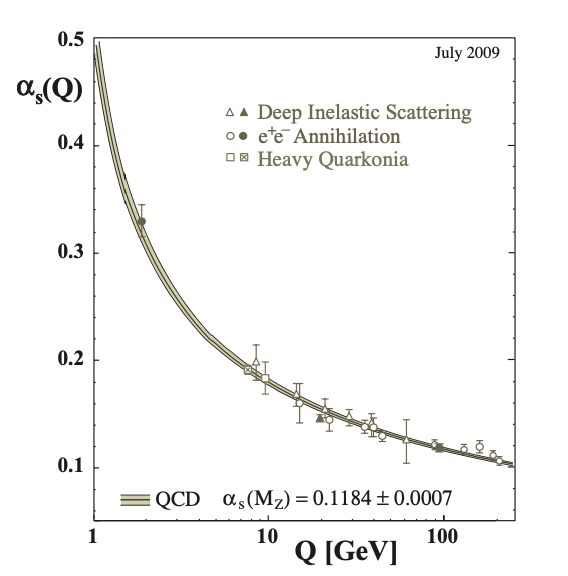
\includegraphics[width=8cm]{../images/asymptotic_freedom.png}
	\caption{Measurements of the strong coupling constant $\alpha_S$}
	\label{alpha}
\end{figure}
\begin{equation}
	\label{QCD fact}
	d\sigma = \sum_{a,b}\int_0^1 dx_a dx_b \sum_F \int d\Phi_F f_{a/h_1}(x_a,\mu_F) f_{b/h_2}(x_b,\mu_F)  d\hat{\sigma}_{ab \rightarrow F} \ ,
\end{equation}
where the sum over $a$ and $b$ runs over all the partonic constituents of the two hadrons $h_1$ and $h_2$ and the inner sum over $F$ runs over all the possible final states $F$

\subsection{Need for MC integration in HEP}
The theoretical framework presented in the previous sections shows us that to make a prediction we need to solve complicated integrals. 

The integrals will become more difficult to evaluate as we approach higher levels of precision. As shown in Eq.~\ref{QCD fact}, we first need to compute the partonic level cross section  $d\hat{\sigma}_{ab \rightarrow F}$ for each possible final state $F$ and for each possible partonic constituents of the hadrons involved in the collisions $a$ and $b$. The partonic cross section is computed at fixed order by integrating the squared matrix element $|\mathcal{M}|^2$ over the phase-space density $d\Phi_n$ (Eq.~\ref{partonic cross section}). For high order terms we obtain difficult mathematical expressions, due to the more intricate Feynman diagrams accessible to the process, that need to be integrated over high-dimensional phase-space, depending on the number of outgoing particles. Moreover, we may be interested in particular kinematics cuts that can further complicate the evaluation of the integral. Finally, if we are interested hadronic-level computations we will need to perform a convolution over the PDFs for each partonic constituents.
%The complexity of the integrals will increase as we approach higher levels of precision since there will be more Feynman diagrams to consider. Moreover, the Feynman diagrams will be more intricate leading to difficult mathematical expressions.

The aforementioned integrals can be solved analytically only if we are dealing with the first perturbative terms of a simple process. Eventually for one dimensional integrals we can use also tools such as the language program \texttt{Mathematica} \cite{Mathematica} to solve such integrals analytically. However, the majority of the calculations performed nowadays involves integrals in high dimensions that cannot be solved analytically or for which the analytical result is often not known.

This is a common problem also in other sectors of physics. The solution is to switch to a numerical approach in order to solve the integrals. This is why we need to use numerical techniques such as Monte Carlo integrators which are particularly suited for complex multi-dimensional integration problems.  



\section{Modern techniques and limitations}

Thanks to the technological development at LHC we are able to obtain experimental data with a very high precision. To test whether 
the SM can explain and predict correctly these data we need to compare them with  theoretical predictions that have the same accuracy.
This leads us to the problem of increasing the precision of the theoretical results. 

As we saw in the previous section, we can obtain an expression for physical observables such as the differential cross section as a series of terms which involves the calculation of high-dimensional integrals. The most relevant technique used to solve these integrals are MC methods, due to the high-dimensions as expected. The problem of reaching higher accuracy is therefore related 
to the possibility of reducing the MC estimate of the variance of the considered integral.

In Section \ref{redu_var} we already discussed some MC techniques that enable us to reduce the variance, however, in the particular case of HEP integrands the task of variance reduction can become problematic.

\subsection{Problems of HEP integration}
One of the first problems when predicting physical observable based on a quantum field theory, such as QCD, is the fact we need to compute the observable beyond the LO term in order to match the experimental data. 

Even if we start with a process with a relatively small dimensional phase space  at LO, the next terms in the perturbation series will involve the computation of integrals with more complicated functions which are defined in a higher dimensional phase-space.

In particular the dimensionality of the integral will increase s.t.:
\begin{itemize}
	\item if we consider a real emission  the phase-space will change from a $3 n$ integration volume to a $3(n+1)$ integration volume
	\item if we consider a virtual emission, we will need to compute an integral of dimension $3n +4$, where $3n$ comes from the phase-space integration and $4$ from the integration over the loop-line
\end{itemize}

Secondly the squared matrix element $|\mathcal{M}^2|$ can become difficult to sample even for common low-dimensional SM processes, since 
in general is particularly peaked in a small region of the integration domain in the vicinity of kinematic divergences. These regions become even smaller for high-dimensional integrands due to the large number of parameters.

This tendency of having sharp peaks in limited regions is the cause of the terrible statistical convergence of naive MC integrators which 
perform uniform sampling. Thus importance sampling techniques are the solution of choice, since they enable us to perform a more effective 
sampling.

Once we have chosen a sampling technique we can reach better accuracies by simply increasing the size of the sample, since, as we have seen, the 
standard deviation for a MC simulation decreases with the size of the sample as $N^{-1/2}$.

Therefore we expect that for each physical process there will be a number of samples needed in order to reach the target accuracy required. 
In particular we will need large samples to reach high target accuracies when dealing with NLO terms due to the high-dimension and the 
complexity of the squared matrix element $|\mathcal{M}|^2$.

However this is only valid from a theoretical point of view, in practice these calculations are performed by computers which can have a hard time
in sampling these complicated integrands as well as dealing with huge samples in order to reach the target accuracy.
In particular the problem related to the CPU cost and the long computational times has been getting a lot of attention over the last years.



\subsection{CPU costs and computational times}
\label{cost}
The CPU cost of MC methods is one of the biggest problem that is driving the budget of big experiments such as ATLAS or CMS.
Since 2010, MC integration has gone from being a trivial element of an experiment's CPU budget to, particularly in the case of top 
quark production processes, an important consumer of up to 20\% of the experiment's CPU budget \cite{Buckley:2019wov}. 
The main driver for this CPU usage has been the availability of the complex multileg and NLO QCD processes. 

This trend of high CPU resources  is in contrast with the CPU budgets currently available at the LHC experiments.   
From Figure \ref{CPU cost} we can see that the annual CPU consumption will overcome the CPU budget especially in Run 4 and Run 5 of the ATLAS
experiment. 
The main problem for the ATLAS experiment is the heavy use of the \texttt{SHERPA} \cite{Gleisberg:2008ta} event generator which is demanding more CPU  by comparison with
\texttt{MadGraph5} \cite{Alwall:2014hca} which dominates the CMS simulation budget. 

\begin{figure}[h]
	\centering
	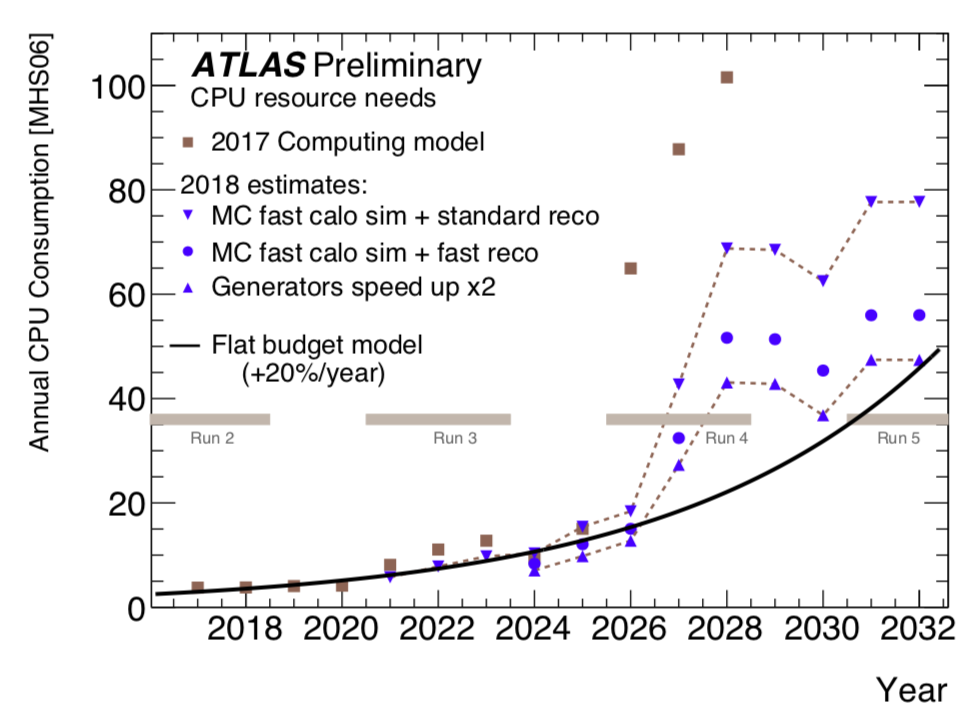
\includegraphics[width = 12cm]{../images/CPU-cost.png}
	\caption{ATLAS CPU resource needs 2018 estimates. Image from Ref.~\cite{ATL-SOFT-PUB-2021-001}.}
	\label{CPU cost}
\end{figure}

Another problem is related to the long computational times.
During a simulation we expect to perform various iterations of our MC routine and the final result 
will be expressed as a weighted average of all the previous outputs.
In particular in the case of integration we need to repeat the process of sampling and the following instructions to compute the integral according to the technique used. When dealing with complex integrands, such as the NLO contribution for a QCD process, sampling could require long computational times.

The current importance sampling techniques can provide an approximate estimate for the sampling distribution by discarding or re-weighting
the samples from such distribution, in particular the aggregation of these imperfect phase-space mappings is one of the major causes for
the poor efficiencies of MC event sampling at high fixed order in the strong coupling $\alpha_S$ .

The ideal distribution would by definition always have unit weights, i.e.\ if the sampling density matches the optimal one, but in practice 
the sample weights have a tail to lower values, since the proposal density includes phase-space points which are not relevant for the integration.
These lower weights can lead to poor statistical convergence in our computations.

 We can also have greater than unit weights, these usually occur when the proposal density underestimates the maximum due to a failure in the
previous sampling, with consequently single-event spikes.

This sample rejection from broad distribution of weights combined with an already CPU-intensive computation of the matrix element explains the huge CPU cost needed in the latest HEP experiments.  From Figure \ref{CPU-time} we can see that the CPU-time per event can become particularly large,  for some current processes it can take up to 24 hours for a single event.


\begin{figure}[]
	\centering
	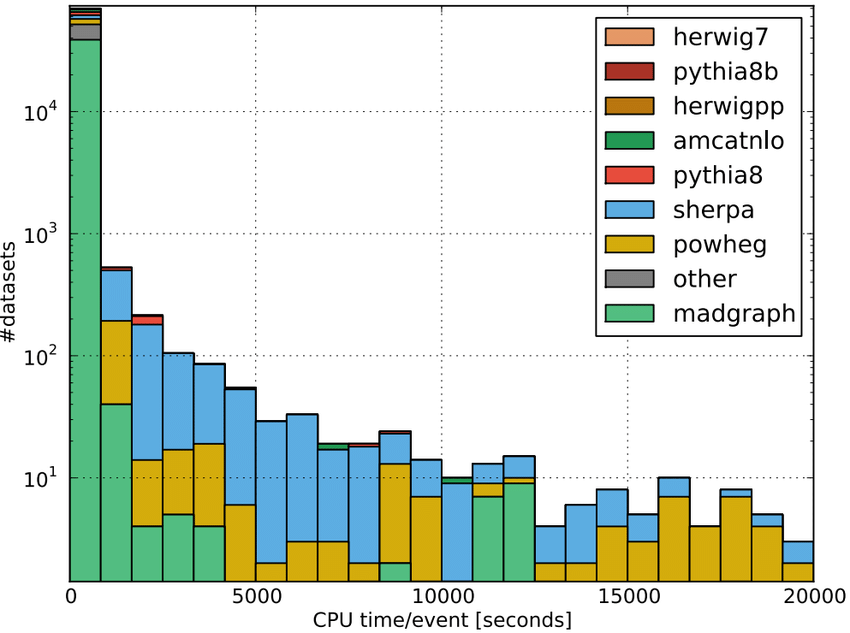
\includegraphics[width = 10cm]{../images/CPU-time.png}
	\caption{CPU time per event using different MC generators. Image from Ref\cite{Buckley:2019wov}.}
	\label{CPU-time}
\end{figure}


\subsection{Possible solutions and aim of the thesis}

The trend of high CPU requirements of the High-Luminosity LHC programme cannot continue, especially because in the future we will need
more precision in the form of 1-loop NLO and 2-loop NNLO QCD calculation that may come at unacceptable CPU costs.

The question is therefore: how can we lower the CPU usage while still achieving high accuracy predictions?
We can work in two different directions in order to achieve our goal.

Firstly, we can develop new algorithms for multi-dimensional integration. In particular new techniques which are able to reach the target accuracy
with a lower number of events thus reducing both the computational times and the CPU usage. These new techniques may include new numerical
MC algorithms as well as ML techniques such as  learning the integration phase-space using boosted decision trees \cite{Bendavid:2017zhk} or deep neural networks \cite{unknown}. 


Secondly, we can lower the CPU usage by looking at new computer architecture such as GPUs or multi-threading CPUs.
 For the purpose of MC integration of the squared matrix element, which comes down to the event sampling and adaptive strategies to compute
 the integral, the use of hardware acceleration devices is particularly appealing. In fact the sampling process is embarrassing parallel since we can
 just use a different random-number generator seed for each run. Also the other operations used in MC techniques such as stratified sampling may
 take advantage of parallelizability due to the fact that we can express the integral as a sum of the MC integration in subregions of the integration volume.
 
 The aim of this thesis is to study and implement new MC integration algorithms with the aim of achieving the target accuracies and at the same time overcoming the computational limitations by taking advantage of hardware acceleration devices.

























 


 









\end{document}